\documentclass[10pt]{article}
\usepackage[margin=1in]{geometry} 
\usepackage{enumerate, xfrac, color, graphicx}
\usepackage{amsmath,amsthm,amssymb,amsfonts,mathabx}
\usepackage{booktabs}
\usepackage{caption}
\usepackage{algorithm}
\usepackage{algpseudocode}
\usepackage{pifont}
\usepackage{listings, courier}
\graphicspath{{/Users/mfzhao/Dropbox/}}
\newcommand{\N}{\mathbb{N}}
\newcommand{\Z}{\mathbb{Z}}
\lstset{breaklines=true, basicstyle=\small\ttfamily, language=R, backgroundcolor=\color{highlight}, stepnumber=5}

\definecolor{highlight}{RGB}{248,248,248}

\begin{document}
	\title{6.867 Problem Set 1}
	\maketitle
	
\subsubsection*{Implementing Gradient Descent}

We implemented a rather naive gradient descent algorithm in Python using an approach similar to the pseudocode below. The function is written in such a way that it can accept arbitrary scalar functions $f$ and their gradients, $\nabla f(x)$, where $x$ can be a vector of arbitrary length, $n$. If $\nabla f(x)$ is not specified, we approximate it using the central differences. The goal of this function is to try and return $\arg\min_x {f(x)}$.

\begin{algorithm}
\caption{Gradient Descent}
\label{GradDescent}
\begin{algorithmic}[1]
\Procedure{Gradient Descent}{}
\State Specify initial guess, step size, and convergence criteria
\State Set current guess equal to initial guess
\While{Distance between last guess and current guess location is greater than convergence criteria}
\State Calculate function at current location
\State Calculate the gradient of function at current location
\State Updated guess = take a step from current guess in direction of gradient proportional to step size
\State Calculate distance between updated guess and current guess
\State Set current guess equal to updated guess
\EndWhile{}
\EndProcedure
\end{algorithmic}
\end{algorithm}

In order to understand the effect of various hyperparameters (our initial guess, the step size, and the convergence criteria) of the algorithm, we compared the results of our gradient descent routine given a number of different parameter combinations for two different functions: $f(x) = \sum_i^n x_i^2$ and $f(x) = \sum_i^n \frac{1}{100}x_i^2 - \cos(x)$. The first of these is a convex function, whereas the second is quite non-convex, with many local minima. A sample of the results of our gradient descent algorithm for numerous values are found below in Table 1.

We find that, in general, the convex function behaves considerably better. Regardless of our initial guess or our learning rate, the algorithm returns a guess in fewer than 1,000 steps, and these guesses are consistently close to $x = (0,0,0,0)$, the "true" value. The final guess' distance from the true value of $x$ is primarily a function of the convergence criteria, which makes sense - the less picky we are with our convergence criteria, the further from the true value of $x$ our final guess will be.

The non-convex function, on the other hand, is much more sensitive to the hyperparameters we specify. The most notable departure from the convex function is the influence of our initial guess. It is much easier for our gradient descent algorithm to get trapped in local minima, and this is clearly illustrated in our results. While this is the most obvious difference, note that changes in both the learning rate and the convergence criteria also lead to non-trivially different guesses for $\arg\min_x {f(x)}$. Note that we do put a cap on the number of iterations allowable, so it is also possible that our non-convex function simply fails to converge, although this doesn't appear to happen in any of the cases illustrated in this text.

Generally speaking, choice of starting value is only important when dealing with non-convex functions, as different starting values may lead to different local extremums. That being said, even for convex functions, good starting values decrease the number of iterations necessary for convergence. Tuning the step size alters the performance of the algorithm, while tuning the convergence threshold alters the accuracy of the algorithm.

It's worth elaborating on the nuances of picking a step size and convergence threshold. For any given convergence threshold, increasing step size will decrease the number of iterations required for convergence. However, we need make sure that the step isn't so large that the algorithm gets caught in a loop where its constantly overshooting the minimum. On the other hand, for a given step size, decreasing the convergence threshold increases accuracy of the algorithm, but it will take additional iterations to reach this higher level of precision. We want to make sure that the convergence threshold isn't so small that we can never converge.

Unfortunately, it might not always be convenient to specify the gradient of our scalar function, $f(x)$, explicitly. It may be complicated to compute, or there may not be a closed form solution. In order to get around this issue, we can approximate the gradient of the function using central differences. We approximate the $i$th element of the gradient, $\nabla_i$, as

\begin{equation}
\nabla_i \approx \frac{f(x_i+h) - f(x_i-h)}{2h}
\end{equation} 

\noindent where $h$ is some small constant (we typically use $h = .001$).

The central difference approximation of the gradient is equivalent to the analytical solution for both the convex and non-convex function. That's great! We also want to know how our gradient descent algorithm compares to more sophisticated optimizers - BFGS and Conjugate Gradient (CG). We compare both the number of iterations and function evaluations required to calculate the minimum of the function. We'll check both the case where we provide an expression for the gradient, and the case where we estimate the gradient. All benchmarking is done with the same starting point: [5, -3, 7, 8]. $f_1(x) =  \sum_i^n x_i^2$ and $f_2(x) = \sum_i^n x_i^{\frac{2}{100}} + \cos(x)$. We see that when passed an analytical solution for $\nabla f(x)$, our algorithm requires about as many function calls, although many more iterations than either BFGS or CG. If we use the central difference approximation for $\nabla f(x)$ instead, our algorithm requires many more iterations and function calls. Later on in this paper, we'll make use of this algorithm to solve some machine learning problems.

\begin{table}
\captionof{table}{Performance of gradient descent given various algorithm hyperparameters} 
\begin{tabular}{llllll}
\toprule
{} &                        $Guess_{i}$ &      step &   Thresh. &    $Guess_{f}$ ($f(x) = \sum_i^n x_i^2$) & $Guess_{f}$ ($f(x) = \sum_i^n \frac{1}{100} x_i^2 - \cos(x)$) \\
\midrule
&    [5.0, -3.0, 7.0, 8.0] &    0.3 &    0.1 &   [0.020, -0.012, 0.029, 0.033] &    [6.150, -0.314, 6.165, 6.176] \\
&    [5.0, -3.0, 7.0, 8.0] &    0.3 &  1e-05 &   [0.000, -0.000, 0.000, 0.000] &    [6.160, -0.003, 6.160, 6.160] \\
&    [5.0, -3.0, 7.0, 8.0] &  0.003 &    0.1 &   [1.172, -0.703, 1.641, 1.876] &    [5.005, -2.999, 6.995, 7.993] \\
&    [5.0, -3.0, 7.0, 8.0] &  0.003 &  1e-05 &   [0.012, -0.007, 0.017, 0.019] &    [6.092, -0.932, 6.200, 6.267] \\
 &   [1.0, -1.0, -3.0, 2.0] &    0.3 &    0.1 &  [0.010, -0.010, -0.031, 0.020] &   [0.007, -0.007, -0.314, 0.024] \\
 &   [1.0, -1.0, -3.0, 2.0] &    0.3 &  1e-05 &  [0.000, -0.000, -0.000, 0.000] &   [0.000, -0.000, -0.003, 0.000] \\
 &   [1.0, -1.0, -3.0, 2.0] &  0.003 &    0.1 &  [0.736, -0.736, -2.207, 1.471] &   [0.995, -0.995, -2.999, 1.994] \\
 &   [1.0, -1.0, -3.0, 2.0] &  0.003 &  1e-05 &  [0.007, -0.007, -0.022, 0.015] &   [0.051, -0.051, -0.932, 0.143] \\
\bottomrule
\end{tabular}
\end{table}

\begin{table}
\captionof{table}{Performance in gradient calculation for analytical and central difference approaches} 
\begin{tabular}{llllll}
\toprule
{} &   $x_{i}$  &  function &   $\nabla_{analytical}$  & $\nabla_{approximate}$ \\
\midrule
&    [5.0, -3.0, 7.0, 8.0] & $f(x) = \sum_i^n x_i^2$ &  [ 10.  -6.  14.  16.] & [ 10.  -6.  14.  16.]\\
&    [5.0, -3.0, 7.0, 8.0] & $f(x) = \sum_i^n \frac{1}{100} x_i^2 - \cos(x)$ & [-0.8589 -0.2011  0.797   1.1494] &[-0.8589 -0.2011  0.797   1.1494] \\
&    [ 1. -1. -3.  2.] & $f(x) = \sum_i^n x_i^2$ &  [ 10.  -6.  14.  16.] & [ 10.  -6.  14.  16.]\\
&    [ 1. -1. -3.  2.] & $f(x) = \sum_i^n \frac{1}{100} x_i^2 - \cos(x)$ & [ 0.8615 -0.8615 -0.2011  0.9493] & [ 0.8615 -0.8615 -0.2011  0.9493] \\
\bottomrule
\end{tabular}
\end{table}

\begin{table}
\captionof{table}{Performance of authors' gradient descent algorithm compared to BFGS and CG}
\begin{tabular}{llllll}
\toprule{} & algorithm & $f_1(x)$ function calls & $f_1(x)$ iterations &  $f_2(x)$ function calls &  $f_2(x)$ iterations \\
\midrule
  & BFGS & 24 & 2 & 78 & 10 \\
  & CG & 30 & 2 & 78 & 6 \\
  & Gradient Descent (analytical) & 20 & 10 & 48 & 24 \\ 
  & Gradient Descent (approximate) & 100 & 10 & 240 & 24 \\
\bottomrule
\end{tabular}
\end{table}

\subsubsection*{Linear Basis Function Regression}

We now consider the linear combination of basis function class regression models. We first derive the maximum-likelihood estimator for the weight vector $\theta$. Note that if we assume Gaussian errors, that is $Y \sim N(X\theta, \sigma^2)$, then our maximum-likelihood estimator is equivalent to the OLS estimator. Hence:
\begin{equation*}
	\hat{\theta}_{ML}=\hat{\theta}_{OLS}=(\Phi^T \Phi)^{-1}\Phi^T Y
\end{equation*}
where $\Phi$ denotes the polynomial basis expansion of $X$.

Using this closed form solution, we determined the maximum-likelihood weight vector for the polynomial basis expansions of $X$ of orders 0, 1, 3, and 9. Using these estimated weight vectors we obtained very similar plots to Bishop as seen below:

\begin{figure}[ht]
	\centering
	\begin{minipage}[b]{.24\linewidth}
		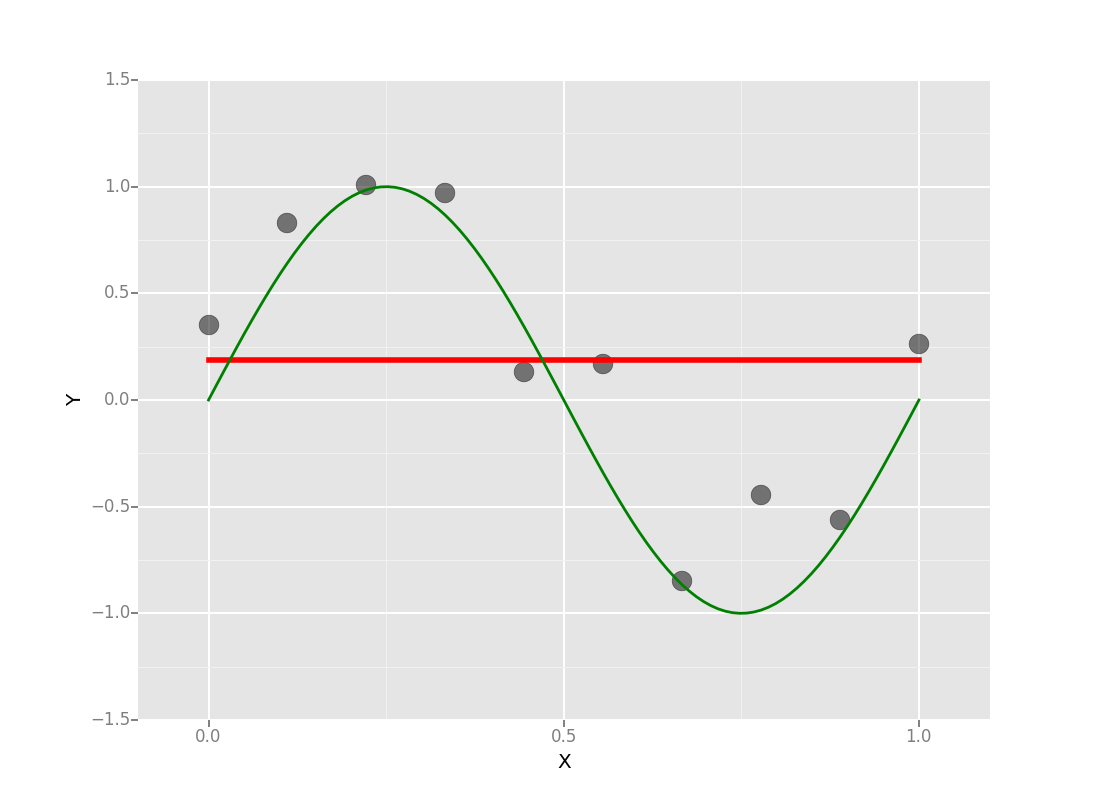
\includegraphics[width=1\linewidth, height=1in]{Meq0.png}
		\caption*{$M=0$}
	\end{minipage}
	\begin{minipage}[b]{.24\linewidth}
		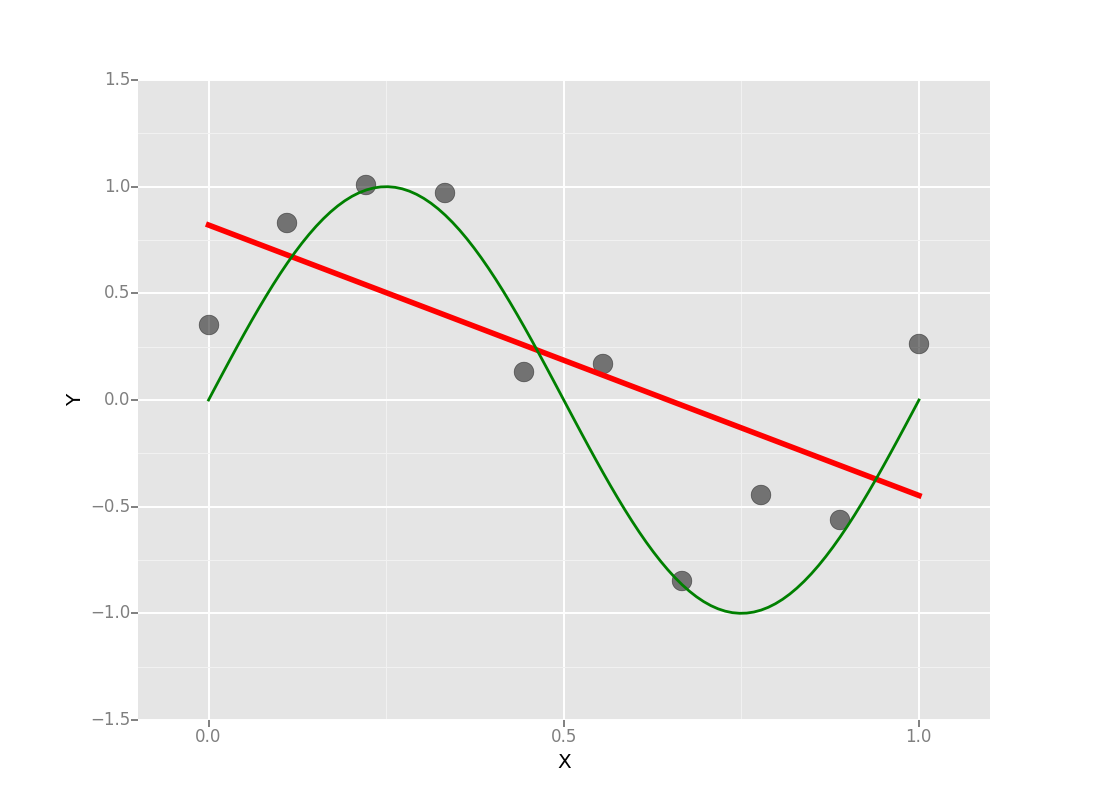
\includegraphics[width=1\linewidth, height=1in]{Meq1.png}
		\caption*{$M=1$}
	\end{minipage}
	\begin{minipage}[b]{.24\linewidth}
		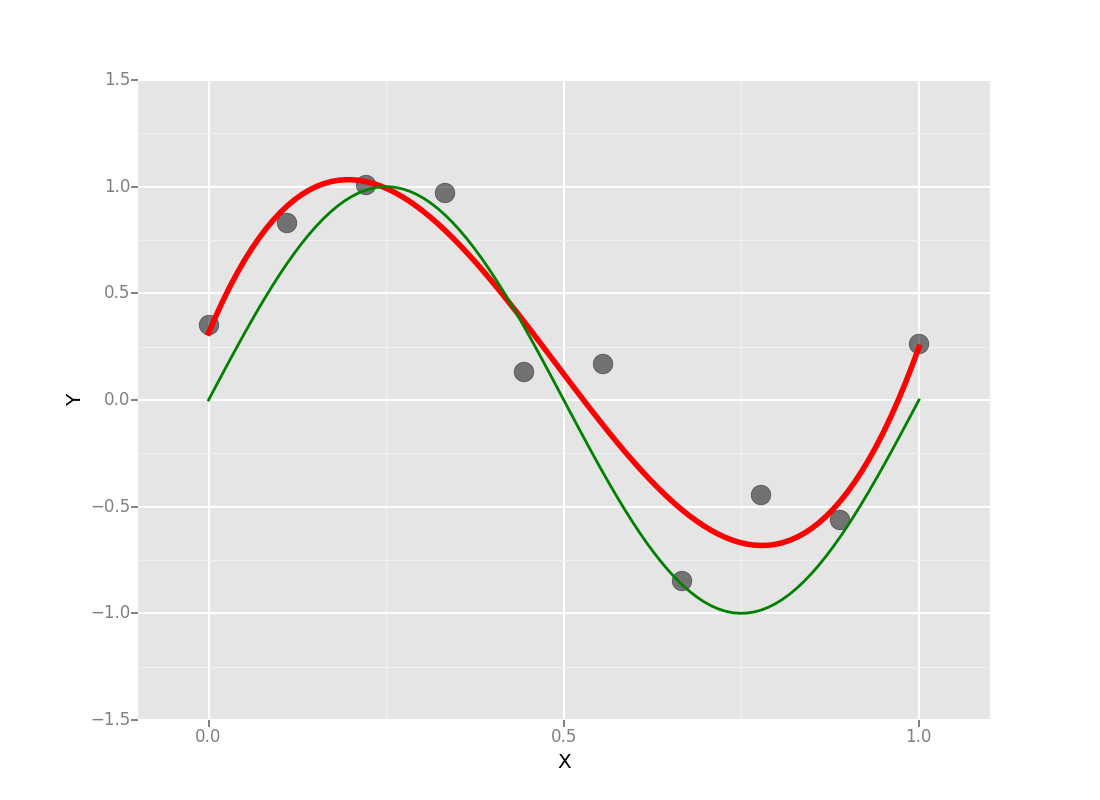
\includegraphics[width=1\linewidth, height=1in]{Meq3.png}
		\caption*{$M=3$}
	\end{minipage}
	\begin{minipage}[b]{.24\linewidth}
		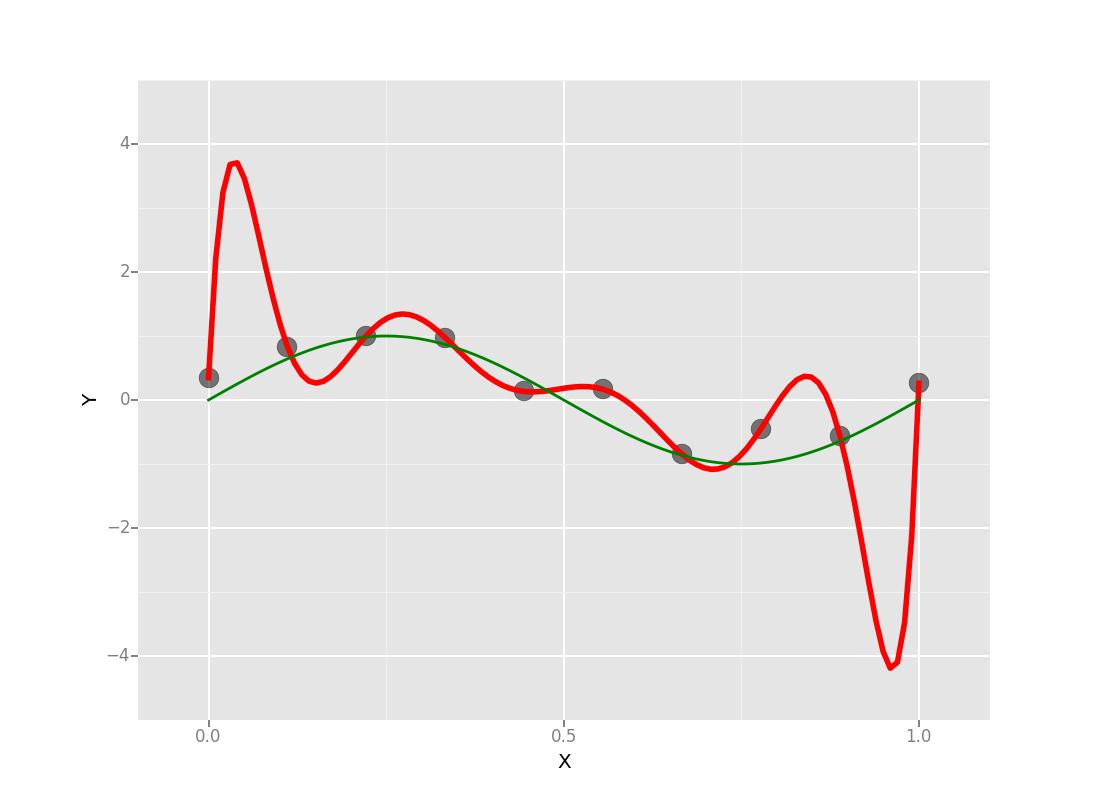
\includegraphics[width=1\linewidth, height=1in]{Meq9.png}
		\caption*{$M=9$}
	\end{minipage}
	\caption{Plots of polynomials having various orders $M$, in red, fitted to the the observed points. The green curve shows the DGF $\sin(2\pi x)$.}
\end{figure}

\begin{table}[ht]
\centering
\captionof{table}{Optimal Weight Vectors for Various Polynomial Basis Expansions of $\mathbf{X}$}
\begin{tabular}{lrrrr}
\toprule
{} &     $M=0$ &     $M=1$ &      $M=3$ &           $M=9$ \\
\midrule
$\theta_0$ &  0.186299 &  0.820212 &   0.313703 &        0.349482 \\
$\theta_1$ &        & -1.267826 &   7.985371 &      232.682435 \\
$\theta_2$ &        &        & -25.426102 &    -5329.068232 \\
$\theta_3$ &        &        &  17.374077 &    48633.377984 \\
$\theta_4$ &        &        &         &  -231944.259392 \\
$\theta_5$ &        &        &         &   640871.190655 \\
$\theta_6$ &        &        &         & -1063154.903003 \\
$\theta_7$ &        &        &         &  1043711.192742 \\
$\theta_8$ &        &        &         &  -558375.328325 \\
$\theta_9$ &        &        &         &   125355.027159 \\
\bottomrule
\end{tabular}
\end{table}

The sum of squared errors of a linear polynomial basis model is defined by: 
\begin{equation*}
	SSE=(\Phi \theta-Y)^T(\Phi \theta-Y),         	\nabla SSE = 2\Phi^T(\Phi \theta-Y)
\end{equation*}
We tested the accuracy of this closed form solution using central differences. The analytical and numerical gradients were essentially identical across many points, even at order $M=9$. This is exactly what we want!

We then applied gradient descent to the SSE function using the analytical gradient to see if we could replicate the plots in Bishop. Optimizing our hyperparameters got increasingly difficult as we increased the order $M$. For $M=0$, we merely needed to tune the step size and we could achieve consistent convergence to the Bishop plot across many different starting values. At $M=1$, we needed to change both the step size and increase the number of maximum iterations before we consistently converged to the optimum. At $M=3$, we also had to tune the convergence threshold to be several order of magnitudes smaller than it was before, and further increase the number of max interations to get consistent convergence. For $M=9$, regardless of how we tried to tune the hyperparameters, we couldn't manage to find a set of hyperparameters that consistently converged, in fact, even scipy's BFGS optimizer failed to consistently produce a plot similar to Bishop's.

As we expected, our naive gradient descent implementation was vastly inferior the scipy's BFGS optimizer. While we could achieve the same level of accuracy as BFGS, our implementation took significantly more iterations. Furthermore, significant time and effort is needed to properly tune our algorithm's hyperparameters, while scipy's BFGS implementation didn't require any tuning. 

Alternatively, we can use a trigonometric basis expansion rather than a polynomial one and get somewhat similar results. We expect that our SSE would converge to 0 as we increased the order $M$. Also, we expect the fit to the "true" data generating function would deteriorate again with increasing order $M$. This is in fact exactly what we see: 

\begin{figure}[ht]
	\centering
	\begin{minipage}[b]{.24\linewidth}
		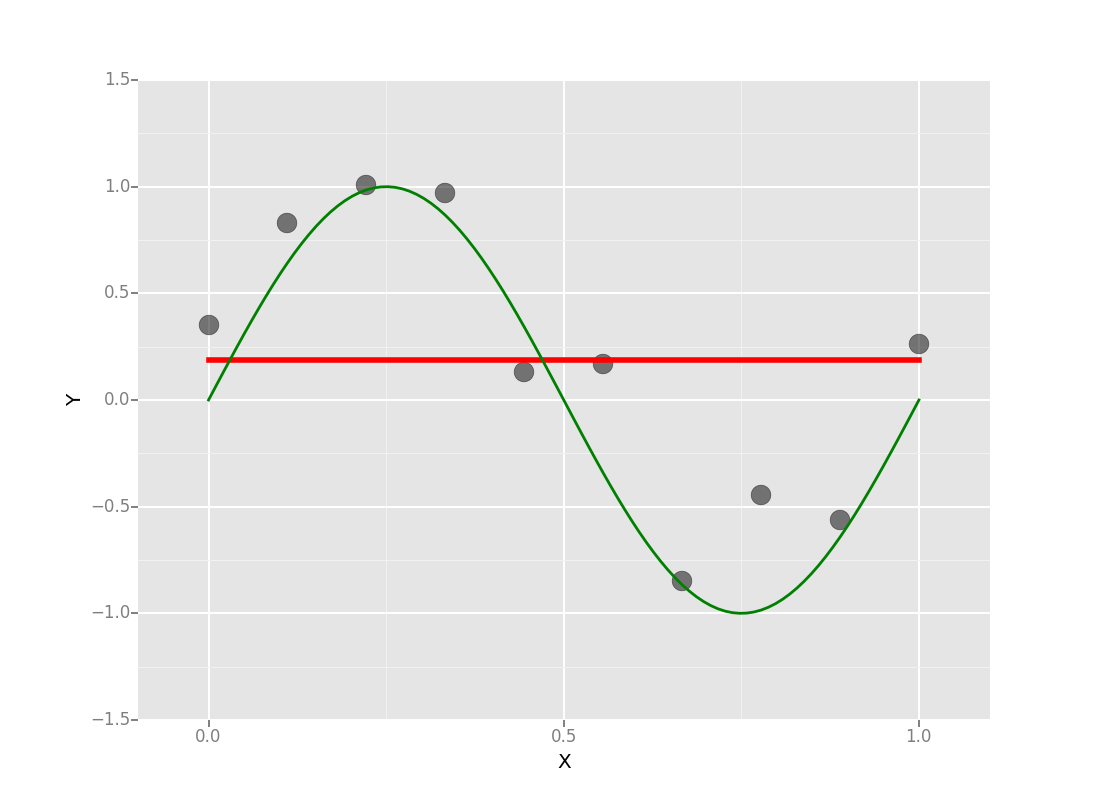
\includegraphics[width=1\linewidth, height=1in]{Meq0T.png}
		\caption*{$M=0$}
	\end{minipage}
	\begin{minipage}[b]{.24\linewidth}
		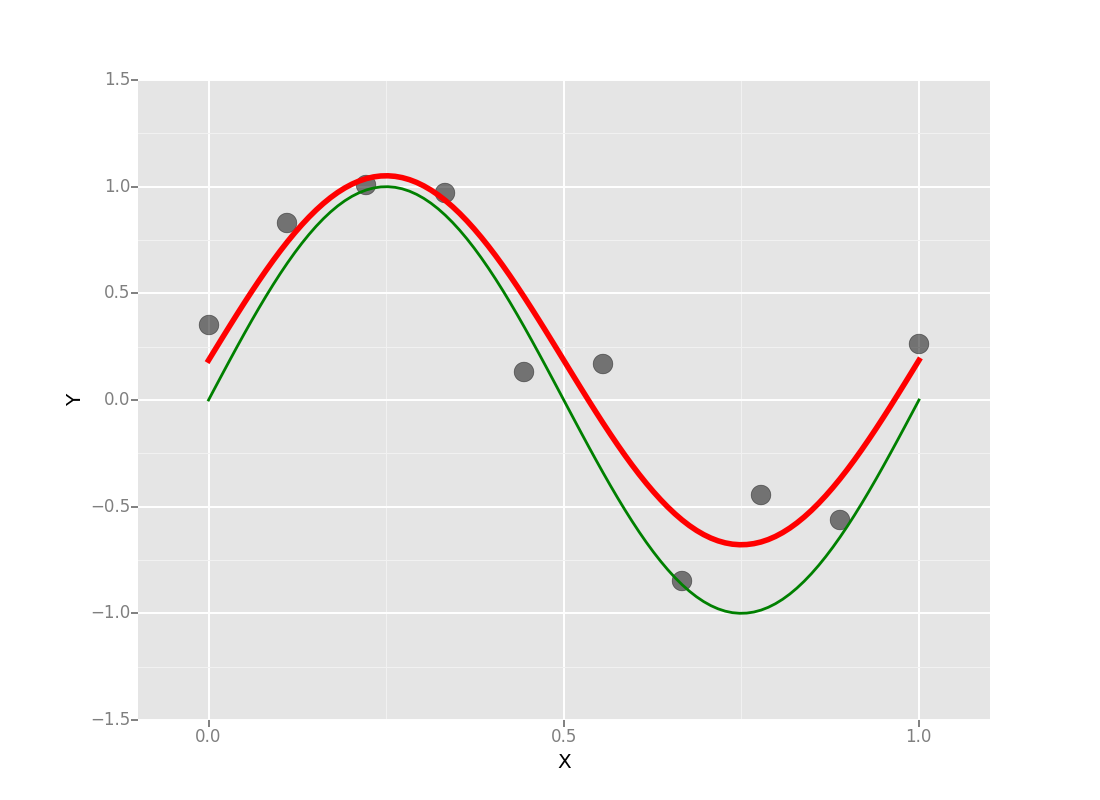
\includegraphics[width=1\linewidth, height=1in]{Meq1T.png}
		\caption*{$M=1$}
	\end{minipage}
	\begin{minipage}[b]{.24\linewidth}
		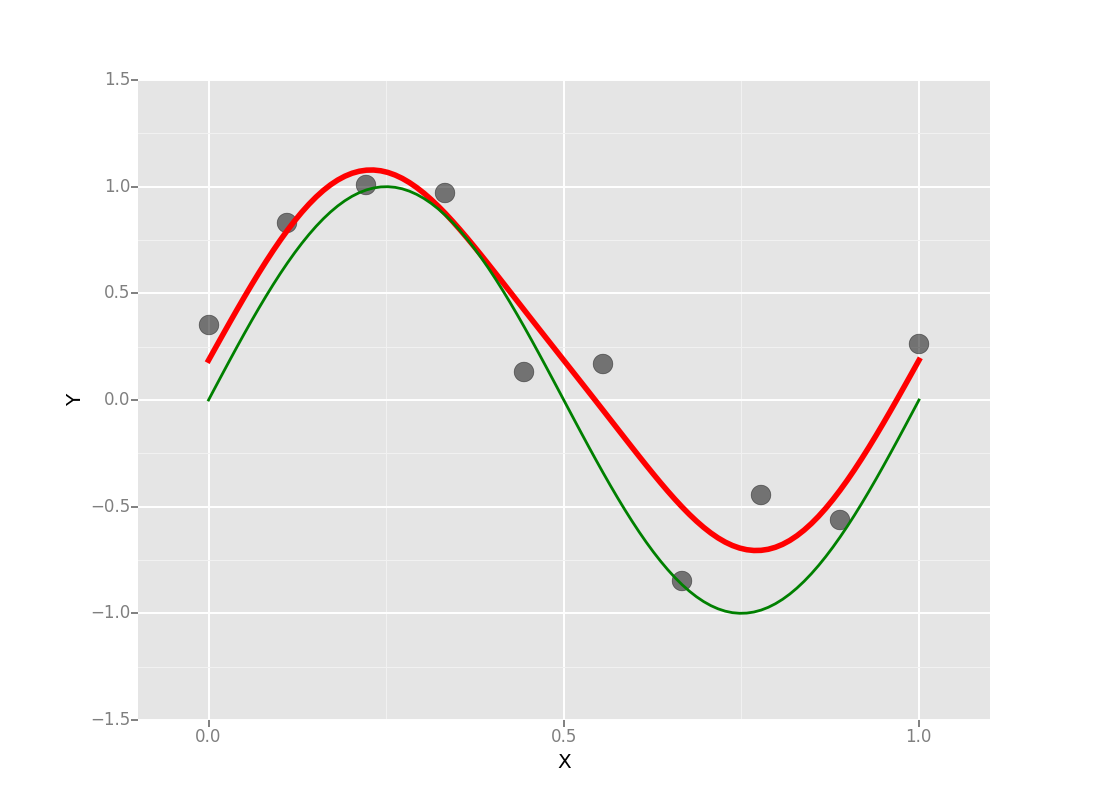
\includegraphics[width=1\linewidth, height=1in]{Meq3T.png}
		\caption*{$M=3$}
	\end{minipage}
	\begin{minipage}[b]{.24\linewidth}
		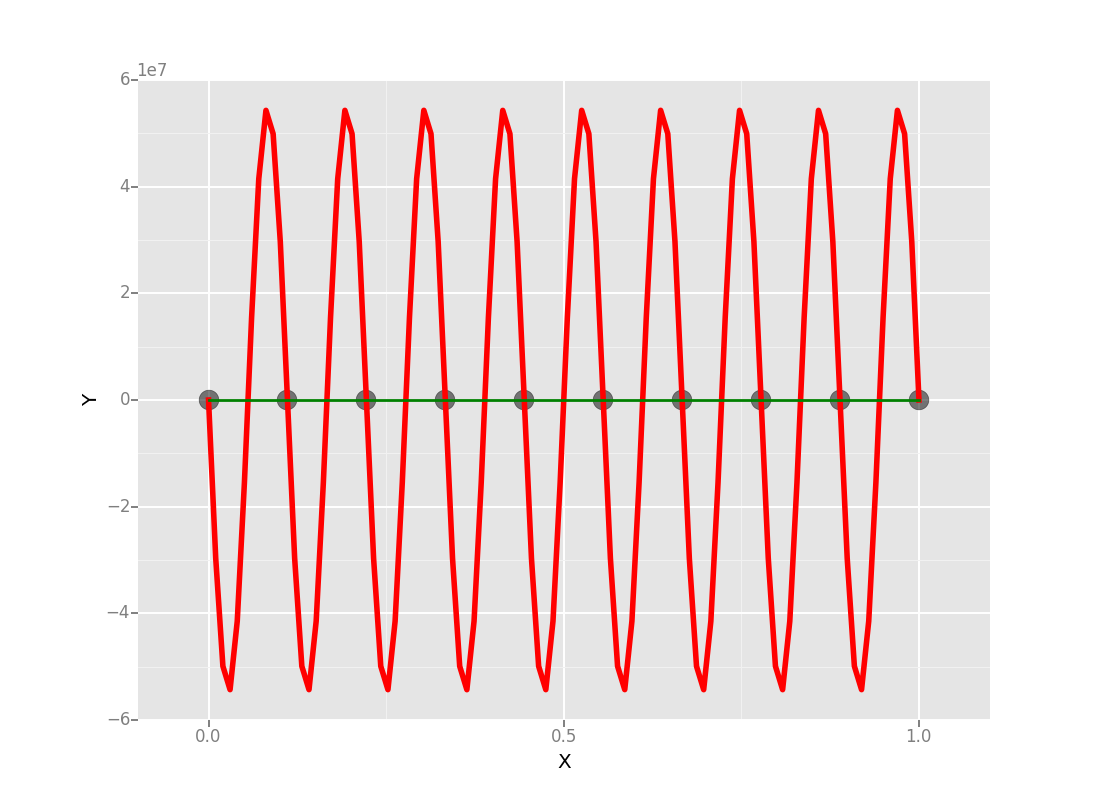
\includegraphics[width=1\linewidth, height=1in]{Meq9T.png}
		\caption*{$M=9$}
	\end{minipage}
	\caption{Plots of trigonometric basis expansions with various orders $M$, in red, fitted to the the observed points. The green curve shows the DGF $\sin(2\pi x)$.}
\end{figure}

Note that orders $M=1$ and $M=3$ provide rather good fits to for the true DGF. We should expect as the the DGF is in fact $\sin(2\pi x)$. However, if we didn't know that this was the true DGF, it might be problematic using a trigonometric basis expansion as it imposes a structure of cyclicality to the fit which may lead to gross misspecification of the model.

\subsubsection*{Implementing Ridge Regression}

Let's now see how regression behaves when we impose a regularization term. The regularization term, $\lambda$, serves to make sure we don't overfit to our training data. We implemented the closed form solution of Ridge Regression in Python, making use of Scipy and Numpy. Note that if you want to test cases where the number of features is greater than the number of data points (something that a well-trained teacher of machine should be skeptical to do), it is useful to use the pseudo-inverse, rather than the inverse to fit your parameters. We learned this the long way after debugging code for hours.

The closed form solution for ridge regression is given by the expression:

\begin{equation}
\hat{\theta} = (\mathbf{X}^T\mathbf{X} + \lambda \mathbf{I})^{-1}\mathbf{X}^t\mathbf{y}
\end{equation}

\noindent where $\mathbf{X}$ is your matrix of features, $y$ is your array of observed values, and $\hat{\theta}$ are your estimated feature weights. $\lambda$ is a regularization parameter, which represents how much you penalize the model for having large feature weights.

Given the data in Bishop 1.4 (which can be seen below), we attempt to fit polynomials of various orders, $M$.  The plot below shows the mean squared error (MSE) that our ridge regression fit gives for values of $M$ between 1 and 5, for values of $\lambda$ ranging from $(10^0 -1)$ to $10^2$. Note that in the case where $\lambda = 0$, we have $OLS$ regression, and as $M$ increases, the model is free to overfit our data. While the MSE on training data is low, if we evaluated this on a new data point, our model would likely perform very poorly. As $\lambda$ gets higher, we penalize the model for having large $\hat{\theta}$ components. Our $MSE$s for these models are relatively large. However, these "large" MSE models are likely to perform better on a new data point!

\begin{figure}[ht]
	\centering
	\begin{minipage}[b]{.48\linewidth}
                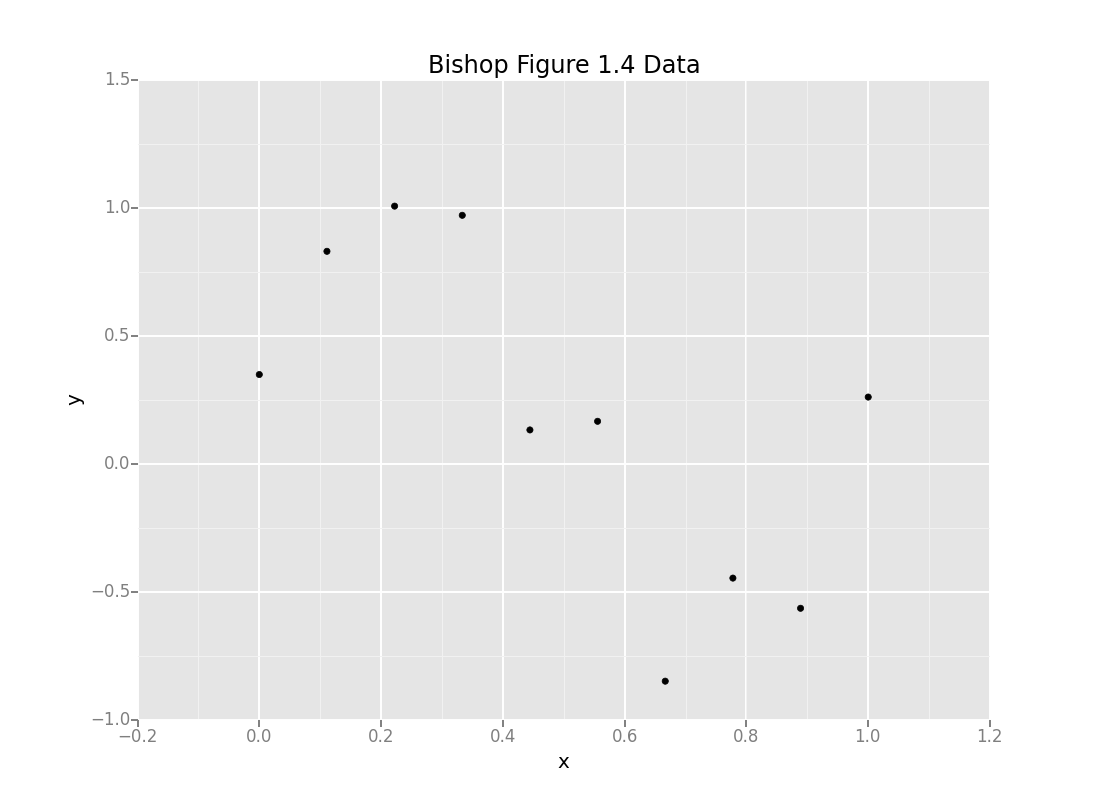
\includegraphics[width=1\linewidth]{Bishop_14_Data.png}
		\caption*{Original Bishop Data}
	\end{minipage}
	\begin{minipage}[b]{.48\linewidth}
                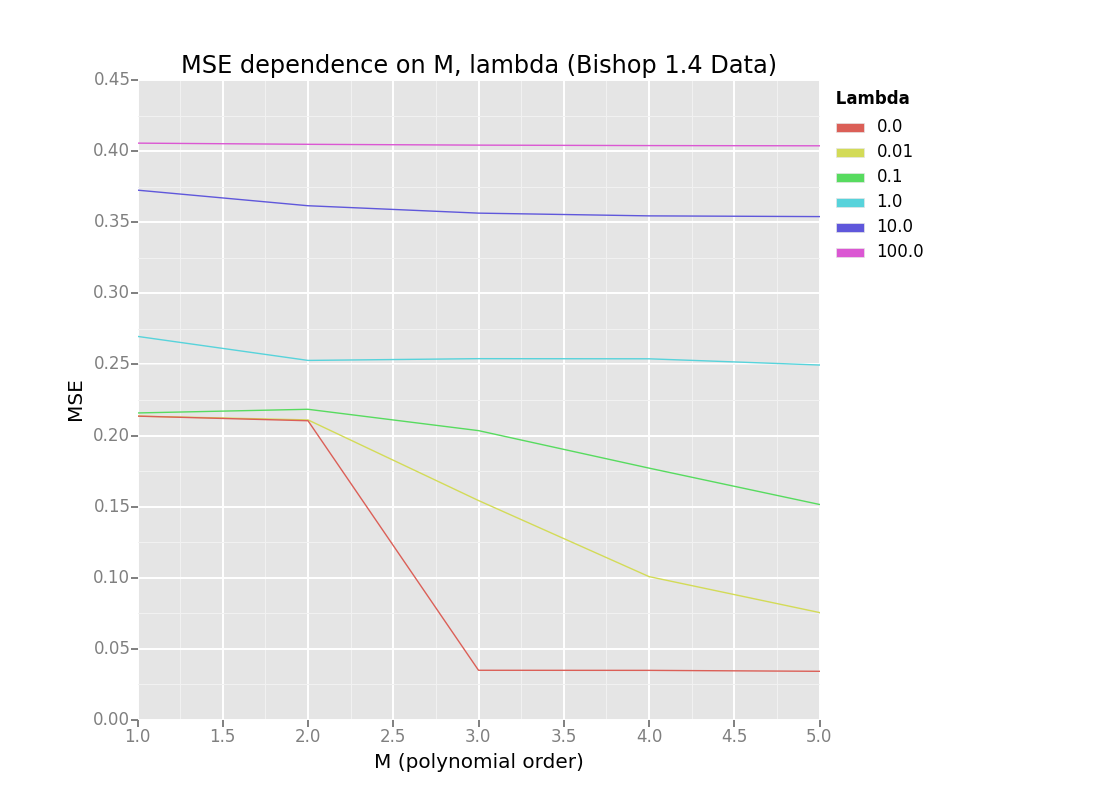
\includegraphics[width=1\linewidth]{MSE_Lambda_Bishop.png}
		\caption*{$MSE$($M$,$\lambda$)}
	\end{minipage}
\end{figure}

In order to avoid overfitting, while making sure that we have chosen values of $\lambda$ and $M$ that make sense, it is common to split the data into a training set and a test set. We will use the closed-form solution for ridge regression to calculate $\hat{\theta}$ on our training set. We will then use that $\hat{\theta}$ to attempt to predict values of $\mathbf{y}$ for the test data. By choosing the $\hat{\theta}$ that is trained on the training data and minimizes MSE on the test data, we are ensuring that we have not overfit our model to the data it is trained on. As one final step in the model selection process, we can check the performance of our final $\hat{\theta}$ on a validation set, to make sure that performance is still good (and we have not overfit to the data in on our test set).

We use this methodology to find the best $\lambda$ and $M$ given three datasets similar to the bishop data. We calculate $\lambda$ and $M$ using the regress\_train.txt, data we validate using regress\_test.txt, and then we test using regress\_validate.txt. We search through a grid of various values for $\lambda$ and $M$, and find that $MSE$ is lowest on the validation set when $\lambda = 1$ and $M = 1$: $MSE = 1.776$ on the validation data set. These parameters gave us an $MSE$ of 1.460 on the training data and and an $MSE$ of 1.415 on the test data. The fact that our $MSE$ is on the same order of magnitude for the test data is a good sign - it indicates that in making sure we didn't overfit to the training data, we didn't accidentally overfit to the validation data.

The $MSE$ for various combinations of $\lambda$ and $M$ on the three datasets (including our chosen set of hyperparameters) is found below. We see that with large $M$ and small $\lambda$, we do great on the training data, but bad on our validation data. For large values of both $\lambda$ and $M$, we do well, but not as well as our optimal values we found through the grid search.

Let's now use this methodology on a real dataset, as opposed to a toy dataset. The dataset that we will use was compiled by Kirsztian Buza at Budapest University of Technology and Economics. It includes 280 numerical values describing a number of blog posts, such as day of week, number of parent pages, and number of comments received within 24 hours. We are hoping to predict the number of comments it will receive in the next 24 hours. This data is split into training, validation, and test datasets, so we will once again perform a grid search to find the value of $\lambda$ that minimizes $MSE$ on our validation set. In this particular case, we are not regressing a polynomial of arbitrary order, so we do not need to test different values of $M$.

We find that for very large $\lambda$ (as large as $10^6$, $MSE$ continues to decrease, although it is always close to 900. A predictor that uniformly predicts the average value of $y$, $\hat{y}$, has an $MSE$ of 1453, so the performance of our model is still better. However, we see that for values of $\lambda$ higher than $10^6$ or so, the value of the MSE increases, and eventually approaches (and eclipses) the MSE of our uniform estimator.

This isn't surprising - the blog feedback dataset is large, with 10,480 observations in the test set. If we interpret the value of $\lambda$ as the strength of our Bayesian prior on our model parameters, it makes sense that our choice of $\lambda$ does not have a substantial effect unless it is significantly larger than the size of our data. Furthermore, the inability of our model to get very low MSE for low $\lambda$ speaks both to the fact that the data has a much higher dimension than our training data, and also suggests that the simple linear model we are using here may not be a very good fit for the data.

\begin{figure}[ht]
	\centering
	\begin{minipage}[b]{.48\linewidth}
                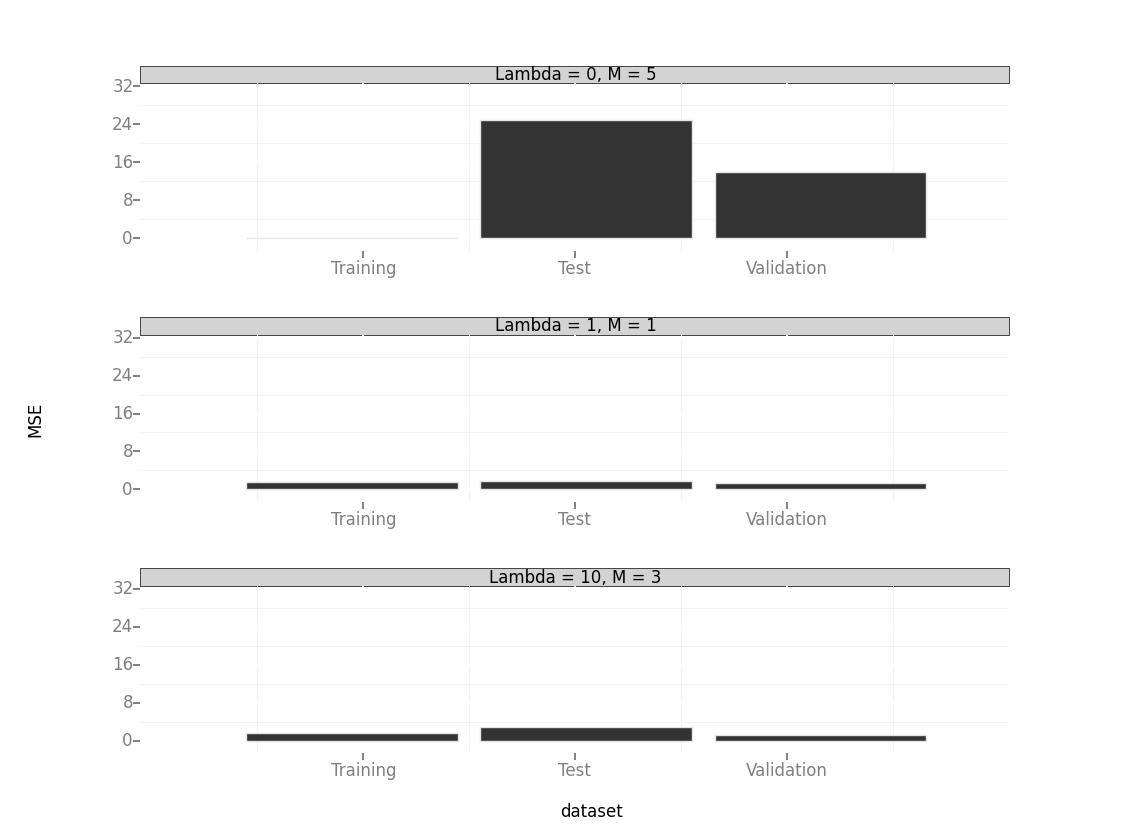
\includegraphics[width=1\linewidth]{MSE_comparison.png}
                \caption*{$MSE$ across different subsets of toy data}                
	\end{minipage}
	\begin{minipage}[b]{.48\linewidth}
                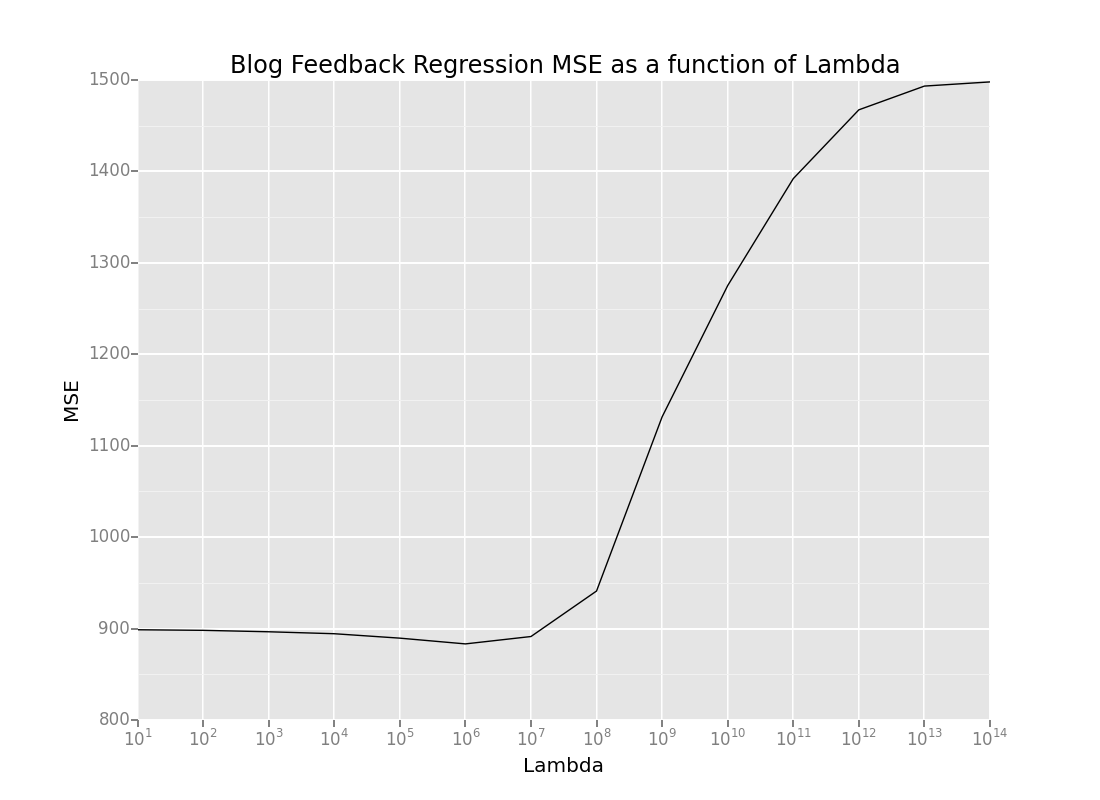
\includegraphics[width=1\linewidth]{BlogFeedbackRegressionMSE.png}
                \caption*{$MSE$($\lambda$) for blog data}
	\end{minipage}
\end{figure}

\subsubsection*{Sparse Regression with LASSO}

Let's now consider the opposite of a 10,480 point dataset - the case where we regress with only 5  training points. For this case, we might consider using LASSO, which penalizes our model with the magnitude of $\lambda$ (as opposed to its squared magnitude). Let's compare LASSO and ridge regression. We first start by determining the optimal penalty $\lambda$ that minimizes the ridge regression $MSE$ on the test set. Our optimal $\lambda$, 0.1, results in an MSE of $0.4395$. When we disable the $L_2$ regularizer, our ridge regression produces the same estimated parameters as OLS, which results in a MSE of $4.0979$. Separately, we determine that $\lambda = .9$ is the optimal LASSO penalty. This results in a $MSE$ of $0.4524$. We plot our 3 obtained fits - OLS, Ridge with $\lambda=0.1$, and LASSO with $\lambda=0.9$ - against the the true DGF.

While its seems the ridge regression fits the true DGF slightly better than LASSO, both these methods vastly outperform standard OLS. We also plot the estimated optimal weight vectors from our 3 models against the true $w$:

\begin{figure}[ht]
	\centering
	\begin{minipage}[b]{.48\linewidth}
                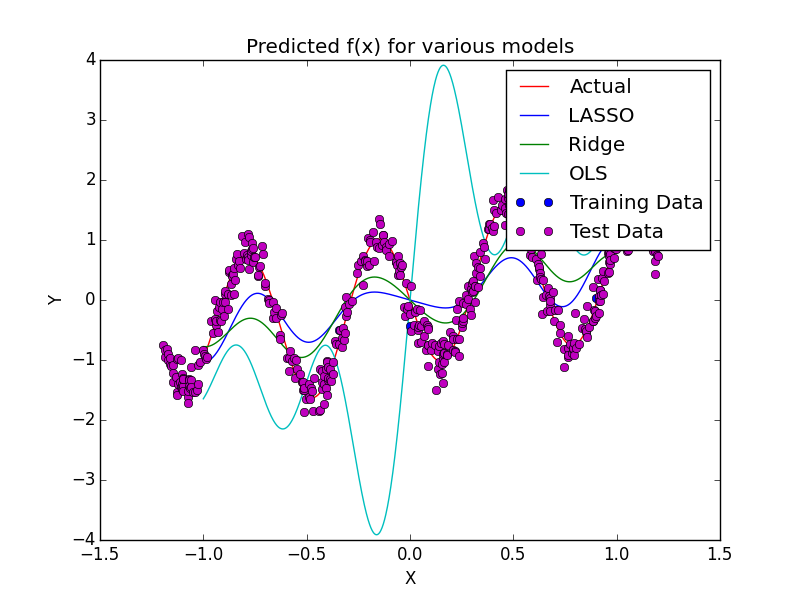
\includegraphics[width=1\linewidth]{plot4}
	\end{minipage}
	\begin{minipage}[b]{.48\linewidth}
                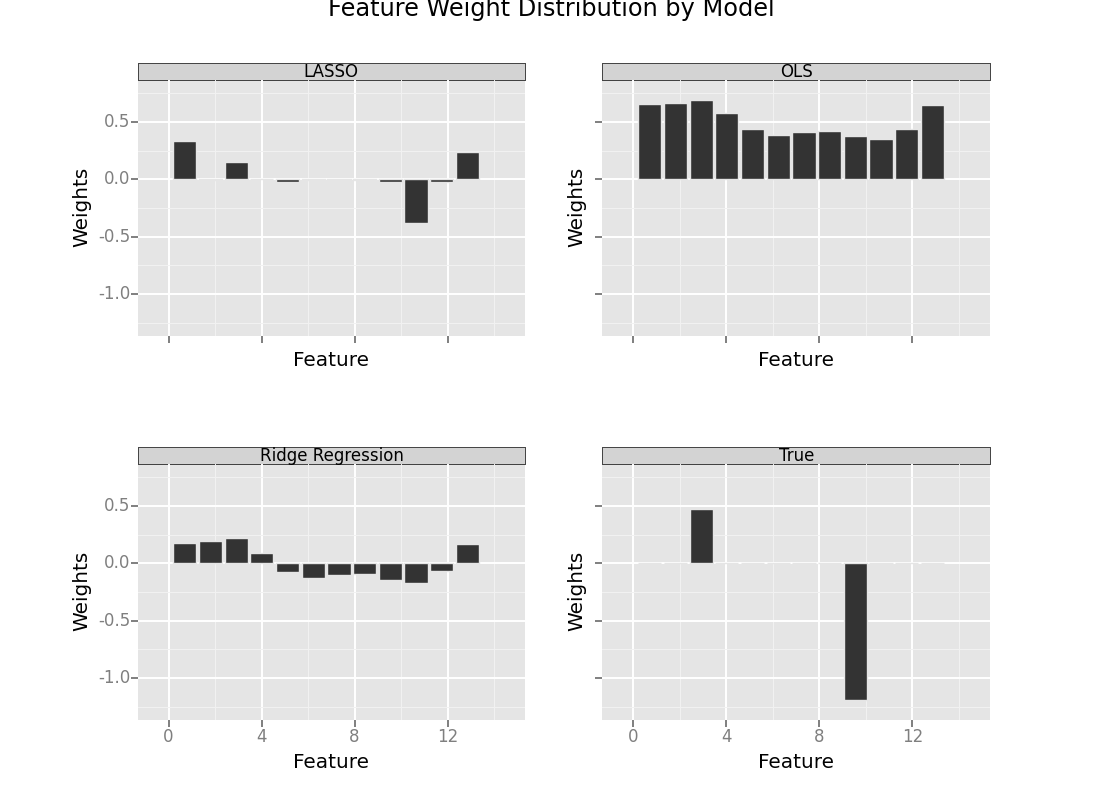
\includegraphics[width=1\linewidth]{Weight_Distributions.png}
	\end{minipage}
\end{figure}

We see that the $L_1$ and $L_2$ regularizers are working as intended! Our ridge regression estimates are considerably smaller than our OLS estimates. Furthermore, our we see sparse estimation from LASSO. This sparsity results from the differences between the $L_1$ and $L_2$ penalty. In ridge regression, we want to minimize the squared error, subject to the constraint that the sum of the weights squared is less than some constant. Geometrically, we can think of this constraint as a sphere of some distance around the origin. In LASSO, we are minimizing the squared error subject to the constraint the the sum of the absolute values of the weights is less than some constant. The $L_1$ constraint can be thought of as a diamond (or regular octahedral) around the origin.

Now consider sets of weights that lead to the the same squared error. These sets can represented as ellipses with the OLS estimates at their center, as that's the point the minimizes squared error. In ridge regression, we're looking for the point where one of these ellipses touches the sphere around the origin, while in LASSO we're looking for the ellipse that touches the diamond. Since the diamond has sharper points, its fairly likely that the ellipse intersects the diamond at one of its points, which represents some weights = 0. It seems that if you expect your weights are sparse, LASSO is the correct regression method to use!

	
\end{document}
Status API Training Shop Blog About Pricing
© 2015 GitHub, Inc. Terms Privacy Security Contact Help